\subsection{Production deployment requirements}
\textit{This section explains what a production deployment is and what requirements must it met.}
~\\
~\\

\subsubsection{Multiple environments in software deployment}
First, it is helpful to distinguish between the terms: \textbf{'infrastructure stack' and 'environment'}. They both may be defined as a collection of infrastructure resources. The difference is that an environment is conceptual, while a stack is concrete. A stack is defined with code, particularly when Infrastructure as Code is applied, and managed using tools. However, an environment serves to fulfill a predetermined purpose. Multiple environments can run an instance of the same system\footnote{\cite{book-iac}, p. 189}.

Typically, there are \textbf{two reasons for which multiple environments are in use}: to support a release delivery process and to run multiple production instances of the system. The first reason allows to have a particular build of an application (e.g. a git commit or a specified version of code) well tested. Such a build has to go through many different environments, e.g.: testing, staging and production. When a build does not pass all the stages in the former environments, it will not be promoted to the production environment\footnote{\cite{book-iac}, p. 190, \cite{book-cicd}, p. 254}. An example release process diagram is depicted below:
\begin{figure}[H]
    \centering
    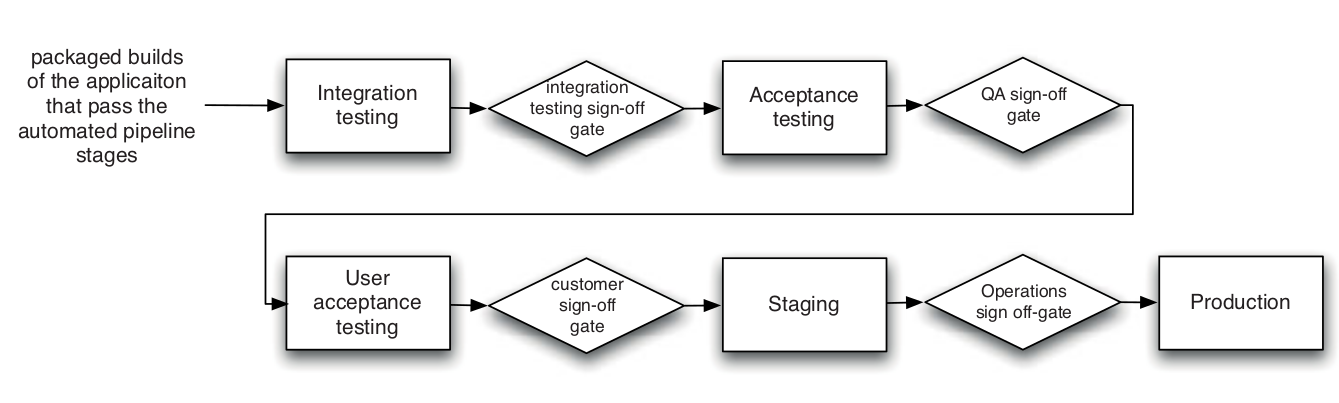
\includegraphics[width=16cm]{figures/cicd-example-release-diagram.png}
    \label{fig:cicd-example-release-diagram}
    \caption{An example test and release process diagram}
    \small{Source: \cite{book-cicd}, p. 255}
\end{figure}

To briefly explain the second reason for multiple environments: they are used in order to ensure fault-tolerance (when one environment fails, the other can take over), scalability (the work can be spread among many clusters), segregation (it may be decided to handle a group of customers using one environment and the other group with the other environment, e.g. for latency purposes)\footnote{\cite{book-iac}, p. 192}.

\subsubsection{Production deployment requirements}
Throughout this work a production deployment means such a deployment which targets the production environment. A list of \textbf{requirements for a production deployment}, gathered through the literature, is provided below:
\begin{itemize}
\item \textbf{Central Monitoring} - this is helpful when troubleshooting a cluster\footnote{\cite{book-mastering-k8s}, p. 41-47, 60, \cite{online-weave-checklists}, p. 5, \cite{online-weave-guide}, p. 2}
\item \textbf{Central Logging} - this is a fundamental requirement for any cluster with number of nodes or pods or containers greater than a couple\footnote{\cite{book-mastering-k8s}, p. 55-58, \cite{online-weave-checklists}, p. 6}
\item \textbf{High Availability} - authors of \cite{book-mastering-k8s} go even further and state that the cluster should be tested for being reliable and highly available \textbf{before} it is deployed into production\footnote{\cite{book-mastering-k8s}, p. 65-80}.
\item \textbf{Live cluster upgrades} - it is not affordable for large Kubernetes clusters with many users to be offline for maintenance\footnote{\cite{book-mastering-k8s}, p. 80}.
\item \textbf{Backup, Quick recovery or even Zero down-time}\footnote{\cite{book-mastering-k8s}, p. 87, \cite{online-weave-guide}, p. 2}.
\item \textbf{Security, secrets management, image scanning} - security at many levels is needed (node, image, pod and container, etc.)\footnote{\cite{book-mastering-k8s}, p. 91-97, \cite{online-weave-checklists}, p. 5, 6, \cite{online-weave-guide}, p. 2, 4-6}.
\item \textbf{Passing tests, a healthy cluster} - "if you don't test it, assume it doesn't work"\footnote{\cite{book-mastering-k8s}, p. 78}
\item \textbf{Automation and Infrastructure as Code} - in production environment a versioned, auditable, and repeatable way to manage the infrastructure is needed\footnote{\cite{book-mastering-k8s}, p. 269, \cite{online-weave-guide}, p. 2}.
\item \textbf{Audit} - to show who was responsible for what action\footnote{\cite{online-weave-guide}, p. 6}
\end{itemize}

\subsubsection{Requirements explanations and how to satisfy them}
\textbf{Monitoring} helps to ensure that a cluster is operational, correctly configured and that there are enough resources deployed. Monitoring is also indispensable for debugging and troubleshooting\footnote{\cite{book-mastering-k8s}, p. 41}. The third reason for using a monitoring system is that historical data is needed for planning purposes. The monitoring strategy should cover four areas\footnote{\cite{book-cicd}, p. 317}:
\begin{itemize}
\item configuring the infrastructure in such a way that it is possible to collect the data
\item storing the data
\item providing dashboards, so that data is presented in a clear way
\item setting up notifications or alarms to let people know about certain events
\end{itemize}
\paragraph{}
Monitoring manages the following data: CPU usage, memory utilization, I/O per disk, disk space, number of network connections, response time, etc. Thus, it is helpful on many different levels: on hardware, operating system,  middleware and application level.
There is a wide range of available open source and commercial tools: Nagios, OpenNMS, Flapjack, Zenoss, Tivoli from IBM, Operations Manager from HP, Splunk, etc.\footnote{\cite{book-cicd}, p. 318}. Solutions recommended for a Kubernetes cluster is: Heapster combined with InfluxDB as backend and Grafana as frontend and there is also cAdvisor\footnote{\cite{book-mastering-k8s}, p. 42, 43}. A nice feature of Grafana are its dashboards. Example Grafana dashboard is presented in the next image:
\begin{figure}[H]
  \centering
  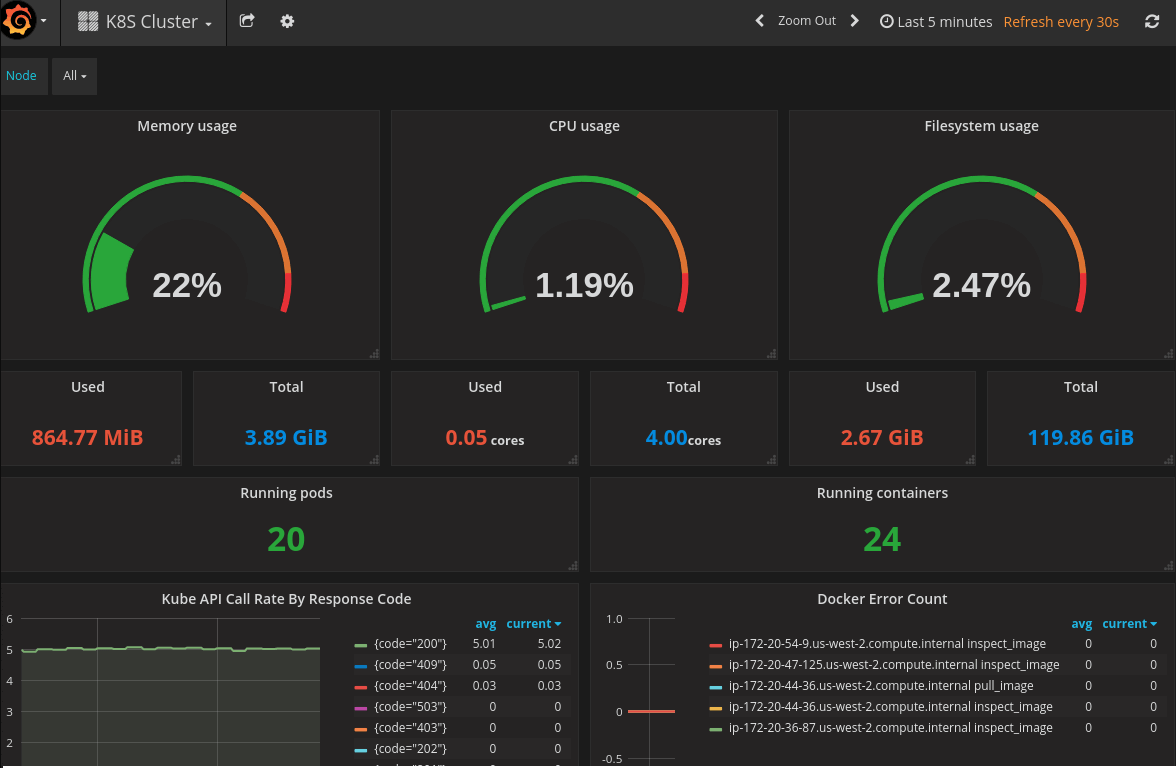
\includegraphics[width=11cm]{figures/grafana.png}
  \label{fig:grafana}
  \caption{Grafana dashboard for Kubernetes cluster}
  \\
  \tiny{Source: \url{https://linoxide.com/linux-how-to/monitor-kubernetes-cluster-prometheus-grafana/}, access: 15.04.2020}
\end{figure}
Grafana also works well with Prometheus, which is a monitoring system and a time series database. Prometheus is also a CNCF graduated project\footnote{\cite{online-prometheus-gh}, \cite{online-prometheus-www}}. When a deployment happens on AWS, another solution for monitoring and logging may be: Amazon CloudWatch\footnote{\cite{online-cw}}. There is also Kubernetes dashboard, which is a built-in solution and doesn't require any customization. Heapster, InfluxDB and Grafana are great for heavy-duty purposes, whereas Kubernetes dashboard is probably able to satisfy the majority of monitoring needs of a Kubernetes cluster\footnote{\cite{book-mastering-k8s}, p. 48}. Example dashboard provided by Kubernetes dashboard is depicted on the next image:
\begin{figure}[H]
  \centering
  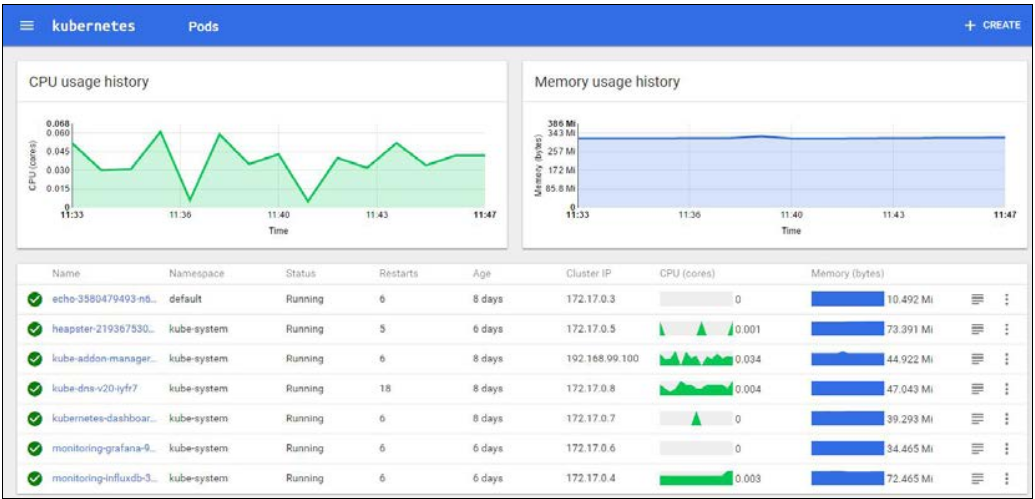
\includegraphics[width=10cm]{figures/k8s-dashboard.png}
  \label{fig:grafana}
  \caption{Kubernetes dashboard in action}
  \\
  \tiny{Source: \cite{book-mastering-k8s}, p. 53}
\end{figure}

Another advantage of Kubernetes dashboard is that it can show \textbf{log messages} of a single container deployed on Kubernetes\footnote{\cite{book-mastering-k8s}, p. 54}. \textbf{Centralized logging} is essential for a production cluster, because usually there are a lot of pods (and containers) deployed, each generating many log messages. It is impossible to require a Kubernetes administrator to log into each container for the purpose of getting the logs. The second reason for the importance of centralized logging is that containers are ephemeral - the log messages kept inside the containers would be lost after a container is redeployed. A popular solution are: Fluentd, Elasticsearch, Kibana\footnote{\cite{book-mastering-k8s}, p. 55-57} and Graylog\footnote{\cite{online-prod-year-k8s}, \cite{online-graylog}}. It is also important to consider that log messages in Kubernetes cluster are generated from many sources: from end-user applications, nodes, Kubernetes system containers and there are also \textbf{audit logs} in the form of e.g. api server events\footnote{\cite{online-graylog-art}}. For the purposes of auditing, when deploying on AWS, one can use AWS CloudTrail\footnote{\cite{online-ct}}.

\paragraph{}
Deploying into testing environment and into production environment differ. However, the same process should be followed, despite of which environment is the target.
